\documentclass{article}
\usepackage{titling}
\usepackage{graphicx}
\usepackage{pgfgantt}
\usepackage{pdflscape}
\usepackage{hyperref}
\usepackage{animate}
\usepackage{movie15}
\renewcommand{\refname}{Kaynakça}
\renewcommand{\figurename}{Resim}

\pretitle{
  \begin{center}
  \LARGE\bfseries
  
\includegraphics[width=0.1\textwidth]{logo.png} % Başlık önüne ekleyeceğiniz bir logo
  \vskip 1em
}
\title{Python ile Derin Öğrenme Kullanarak Otonom Bir Araba Oluşturmak}
\author{Ali Kağan Uyanık}
\date{Mart 2024}

\begin{document}
\begin{titlingpage}
    \maketitle
    \begin{center}
        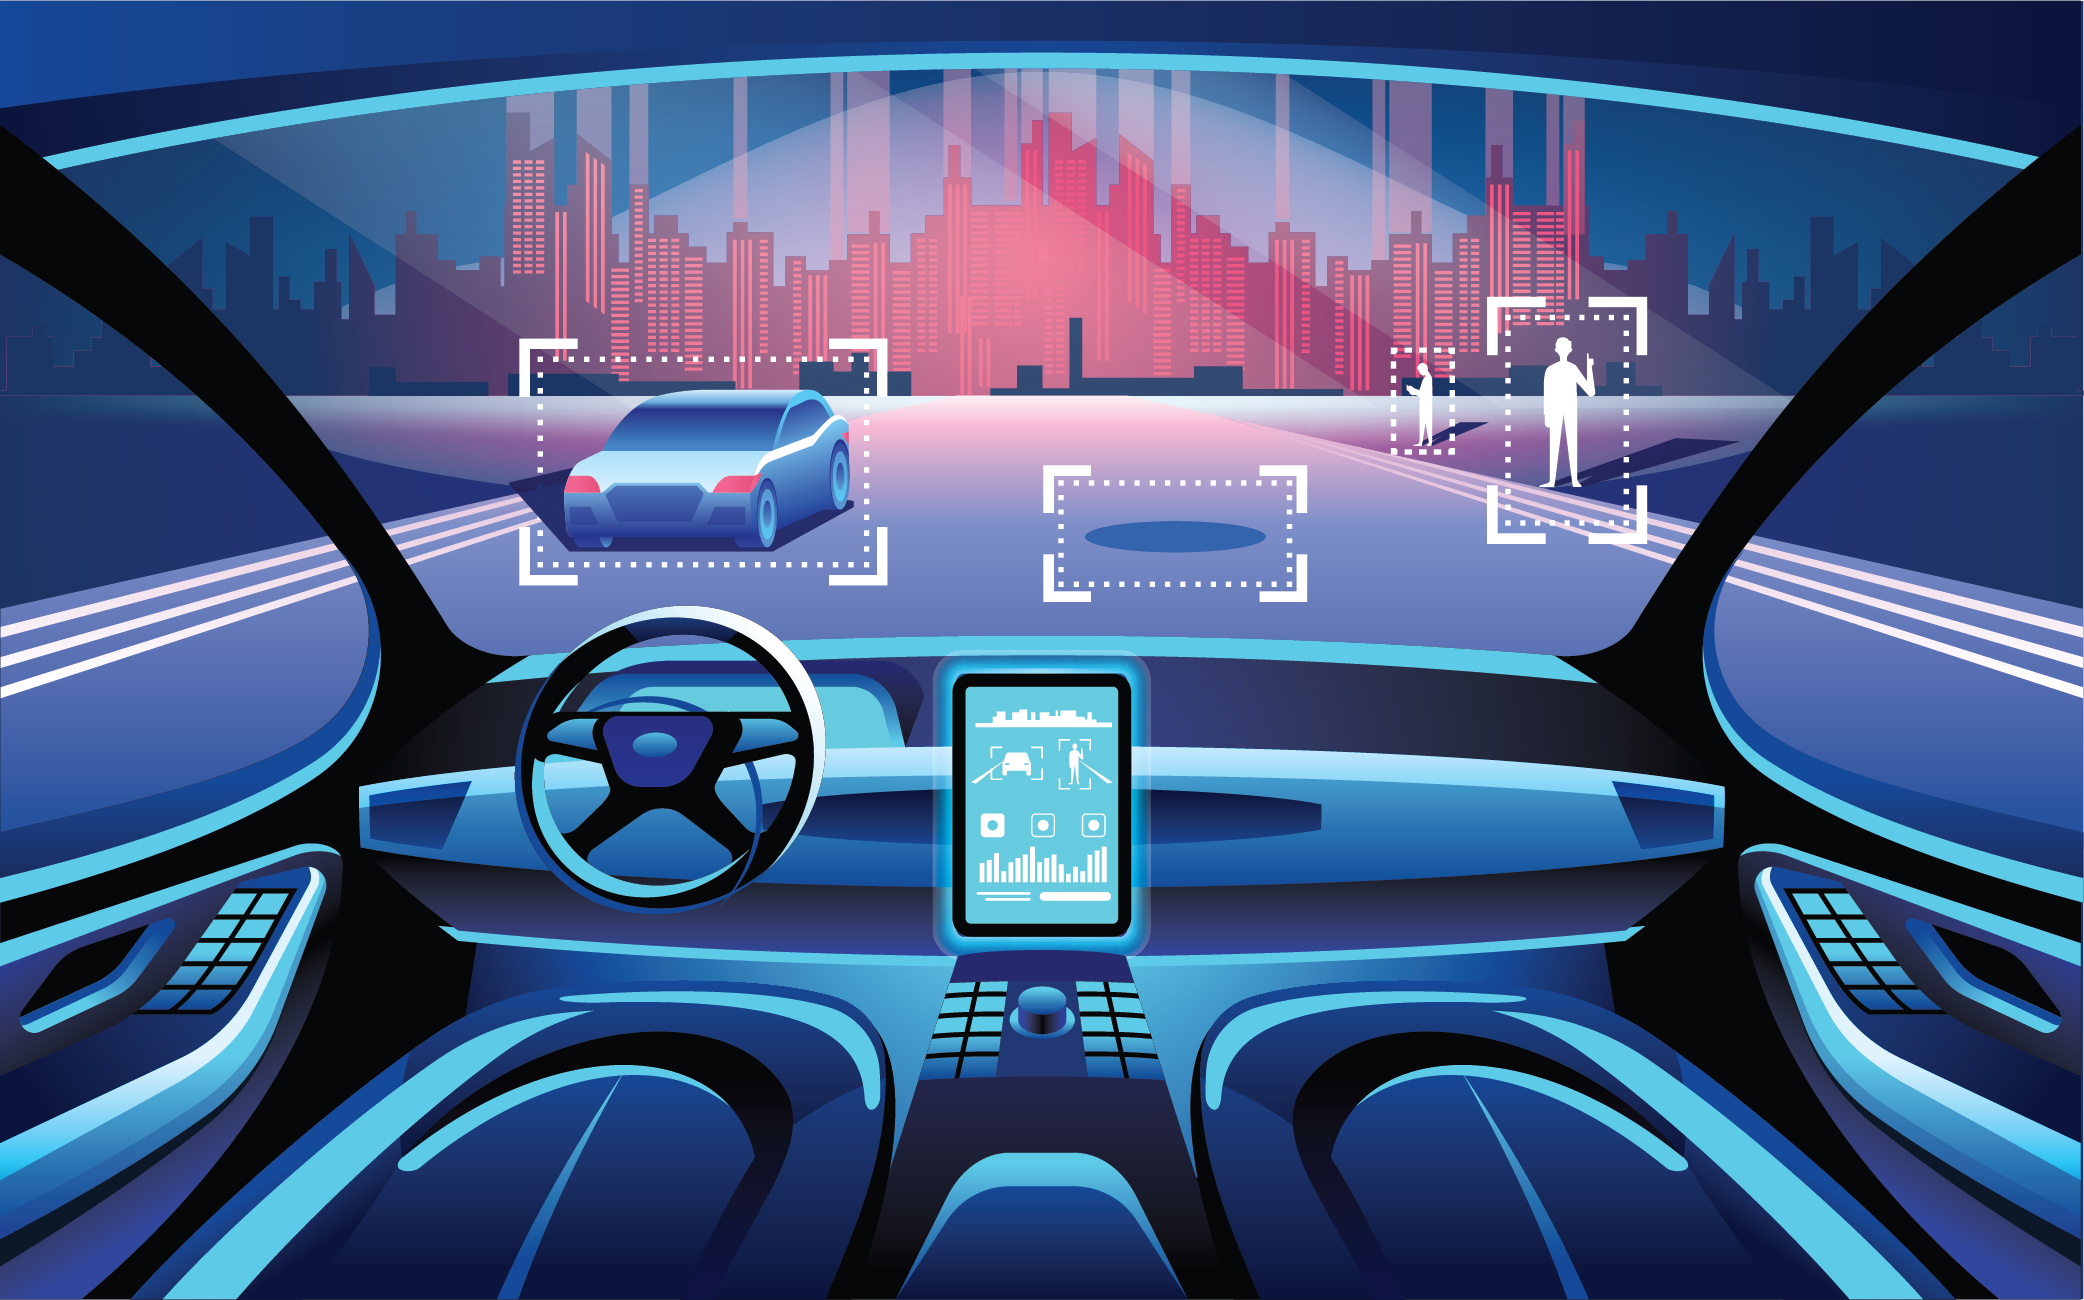
\includegraphics[width=0.8\textwidth]{selfDriving.png} % Araba resminin dosya adını belirtin
    \end{center}
    \vfill
    \rule{\textwidth}{0.5pt}
    \renewcommand{\abstractname}{Özet}
    \begin{abstract}
        \noindent Bu projenin amacı, Python programlama dili ve çeşitli derin öğrenme, bilgisayarla görü ve makine öğrenimi teknikleri kullanarak otonom bir araç geliştirmektir. Otonom aracın çevresini algılamak, kararlar almak ve güvenli bir şekilde hareket etmek için gerekli yeteneklere sahip olması hedeflenmektedir.
    \end{abstract}
    \rule{\textwidth}{0.5pt}
    \vfill
\end{titlingpage}
\newpage
\section{Giriş}
\rule{\textwidth}{0.5pt}\\[10pt]
Teknolojinin hızla gelişmesiyle birlikte, otonom sürüş sistemleri\cite{yiugit2020otonom}otomotiv sektöründe devrim niteliğinde bir değişim başlatmış durumda. Geleneksel sürüş alışkanlıklarını geride bırakarak, araçlar artık kendi kararlarını alabilir, çevrelerini analiz edebilir ve yolculuk boyunca tüm kontrolü ele alabilir hale geldi. Otonom sürüş, sadece bir teknolojik yenilik olmanın ötesinde, günümüz toplumlarının ve insanlığın bir dizi temel ihtiyacına karşılık verebilecek bir potansiyele sahip.\\[30pt]

\noindent Otonom sürüş, günümüzün yoğun ve karmaşık trafik koşullarında insan hatalarını en aza indirerek güvenliği artırma potansiyeli taşıyor. Ayrıca, uzun yolculuklarda sürücülerin yorgunluğunu azaltarak ve trafik stresini hafifleterek konforu artırabilir. Tüm bunlar, otonom sürüşün sadece bireylerin günlük hayatını değil, aynı zamanda şehir planlaması, ulaşım sistemleri ve çevresel sürdürülebilirlik gibi geniş bir perspektiften toplumları etkileyebilecek bir dönüşümü temsil ediyor.\\[30pt]

\noindentİnsanlık, nüfusunun artmasıyla birlikte ulaşım sistemlerine olan talebin de arttığı bir dönemden geçmektedir. Şehirler daha yoğun hale gelmekte, trafik sorunları ve çevresel kirlilik gibi sorunlarla karşı karşıya kalmaktadır. Otonom sürüş teknolojisi, bu zorlukları ele almak için potansiyel bir çözüm olarak ortaya çıkmaktadır. Akıllı sensörler, yapay zeka algoritmaları ve sürekli olarak güncellenen haritalar gibi unsurlar sayesinde otonom araçlar, trafiği daha etkin bir şekilde yönetebilir, kazaları önleyebilir ve karbon emisyonlarını azaltabilir.\cite{chai2021autonomous}\\[100pt]



Aşağıdaki gantt şeması, projenin başlatılmasından sonraki önümüzdeki haftalarda önerilen konseptin ilerlemesine ilişkin proje hedefini temsil etmektedir\\[15pt]

\begin{landscape}
\thispagestyle{empty} % Sayfa numarasını kaldırmak için
    \begin{figure}
     \centering
  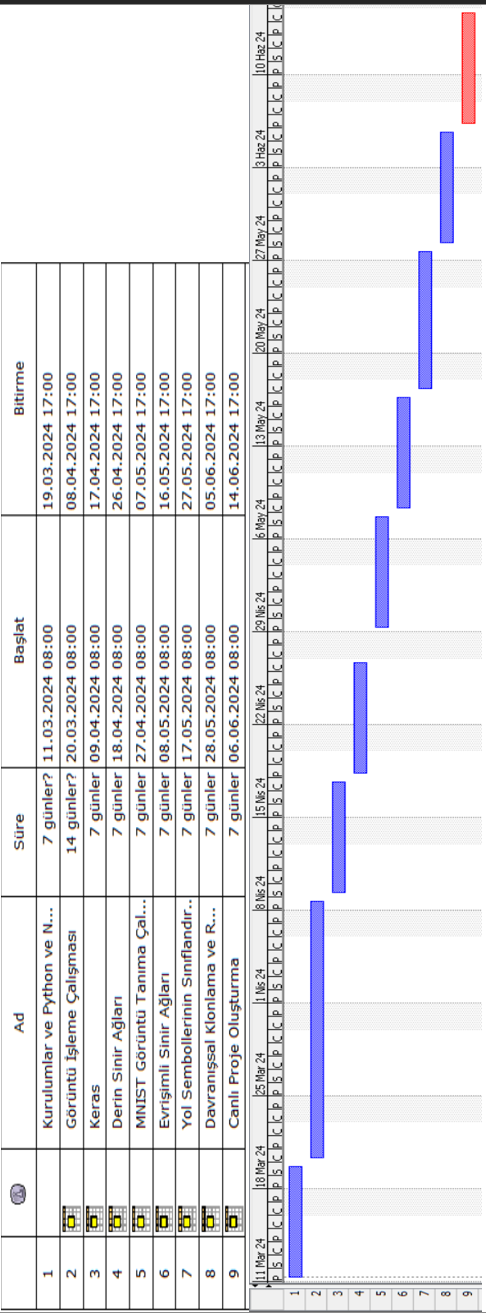
\includegraphics[angle=270,width=1.8\textwidth]{yanchart.PNG}\centering % Resim dosyasının adını ve uzantısını belirtin
  \caption{Gantt Chart}
  \label{fig:resim_etiketi}
\end{figure}

    % Yana çevirmek istediğiniz içerik buraya gelir
\end{landscape}



\newpage


\section{Proje Aşamaları}
\rule{\textwidth}{0.5pt}

\subsection{Kurulumlar ve Python-Numpy}
\subsubsection{Kurulumlar}Anaconda dağıtımının sunduğu çeşitli bilimsel paketleri projemde kullanmaya başlamayı hedefliyorum.Bu paketleri başarılı bir şekilde kurarak, projemin temel altyapısını oluşturmayı düşünüyorum.Ayrıca, bilgisayar görüşü ve davranış klonlaması bölümlerinde kullanacağım metin düzenleyiciyi de kurmam gerekiyor.Bu adım, projenin farklı aşamalarında kullanacağım yazılım araçlarını hazır hale getirmem konusunda önemlidir.
\subsubsection{Python}Bu bölümde, Python programlama dilinin temellerini öğreneceğim.Python, genel amaçlı bir dil olduğu için farklı türde programlar oluşturmak için tasarlanmıştır.Bu kısımda Python ile veri tipleri,aritmetik işlemler,değişkenler,metotlar,listeler,Python slice() kullanımı,Python üyelik (membership) operatörler,Python'da Mutable,en çok kullanılan Python metod ve fonksiyonları,Python Tuple,Pythonda veri yapıları gibi konular hakkında bilgi edinip örnekler yapacağım.
\subsubsection{Numpy}Python'un kendisi, temiz ve okunabilir kod yazmamıza olanak tanır; ancak genel amaçlı bir dil olmasına rağmen, büyük veri setlerinin niceliksel analizini doğrudan yapma yeteneğine sahip değildir.İşte bu yüzden numpy adlı özel bir kütüphaneden faydalanmayı düşünüyorum.Bu bölümde dizi, listeler ve numpy stack() üzerinde çalışmalar yapacağım.\\[15pt]

\subsection{Görüntü İşleme Çalışması}
Bu projenin ana odak noktası derin öğrenme olsa da,projenin birçok bölümünde açık kaynaklı bir bilgisayar görüşü kütüphanesi olan openCV'yi kullanacağım.Eğitim verilerini derin sinir ağına beslemeden önce openCV'yi kullanarak bu verileri ön işlemeyi planlıyorum.Şeritleri tanımlamak için openCV'yi kullanmak,otonom araçların yollarda seyretmesinde temel bir adımdır\cite{madan2022road}.OpenCV'nin sunduğu bazı temel yetenekler arasında kenar tespiti, renk dönüşümleri, morfolojik işlemler ve nesne algılama gibi işlemler bulunmaktadır. Bu işlevler, şeritleri tanımlama gibi karmaşık görevler için temel oluşturur.Bu bölümde,hem openCV'nin yeteneklerini anlamayı hem de derin öğrenme ile nasıl entegre edilebileceğini öğrenmeyi planlıyorum.\\[15pt]
\begin{figure}
  \centering
  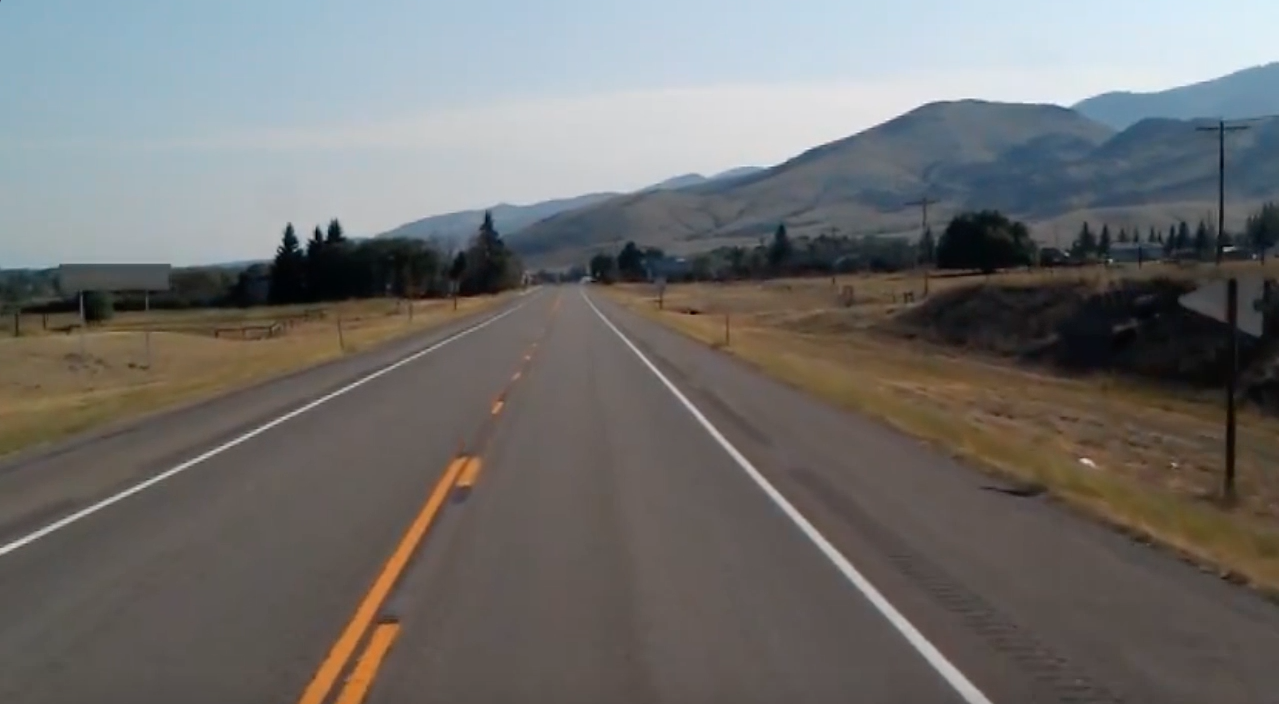
\includegraphics[width=0.9\textwidth]{test_image.jpg} % Resim dosyasının adını ve uzantısını belirtin
  \caption{Resimdeki Şeritleri Tanıtmak için Kullanacağım Örnek Görsel}
  \label{fig:resim_etiketi}
\end{figure}


\subsection{Keras ve Nöral Ağlar}
Nöral ağlar biyolojik nöral ağlardan esinlenmiş ve biz insanların öğrenme şeklini belirsiz bir şekilde taklit etmiştir.En temel nöral ağ formu olan perceptron,bir beynin biyolojik nöronu ile benzerlik gösterir.Perceptron, girdileri giriş düğümleri şeklinde almak ve uygun çıkışı transfer etmek üzere eğitilmiştir. Bu, nöronlarda dendritin elektrik sinyallerini alması ve aksonun uygun sinyali göndermek için birden fazla akson terminaline dallanmasıyla benzerdir.Bu bölümde, bir perceptronun çalışma prensiplerine, ağırlıklara ve gradyan inişi konularına bakacağım.Bir aracın şu anda hangi kısmında olduğuna göre kendi başına sürmesini sağlamak için bir nöral ağ kullanmayı planlıyorum.Bu bölümde,sadece basit bir perceptron temelli ağ oluşturmak için Keras'ı kullanmayı düşünüyorum.\\[15pt]

\subsection{Derin Sinir Ağları}
Karmaşık veri ile uğraşmak için daha karmaşık, derin nöral ağlara ihtiyaç duyuyoruz; çünkü bunlar daha yüksek öğrenme kapasitesine sahiptir.Bunu trafik işaretlerinden görüntü özellikleri çıkarmak için ve aynı zamanda bir otonom araç simülasyonundaki belirli bir yolun kısmından görüntü özellikleri çıkarmak için kullanacağım; böylece uygun direksiyon açısını tahmin etmemize yardımcı olacak.\\[15pt]
\subsection{MNIST Görüntü Tanıma Çalışması}
Mnist veri seti ve derin nöral ağları kullanarak bir modelin görüntü verisine uygun olmasını nasıl sağlayacağımı öğrenmeyi planlıyorum..\\[15pt]

\subsection{Konvolüsyonel Sinir Ağları(CNN)}Konvolüsyonel Sinir Ağları,görüntü sınıflandırma için gidilecek model haline gelmiş, yapay sinir ağlarını geride bırakmıştır.Konvolüsyonel sinir ağlarıyla resimleri nasıl sınıflandıracağımızı öğrenmeyi ve yüksek bir doğruluk oranıyla bu işi yapmayı planlıyorum.\\[15pt]

\subsection{Yol Sembollerinin Sınıflandırılması}Trafik işaretleri, 43 farklı sınıf arasında sınıflandırılabilen verilerdir.Veri setlerini ön işlemek ve hazırlamak, derin öğrenme alanında son derece önemlidir\cite{saadna2019speed}.Şimdiye kadar öğrendiğim her şeyi bir araya getireceğim.\\[15pt]

\begin{figure}[h]
  \centering
  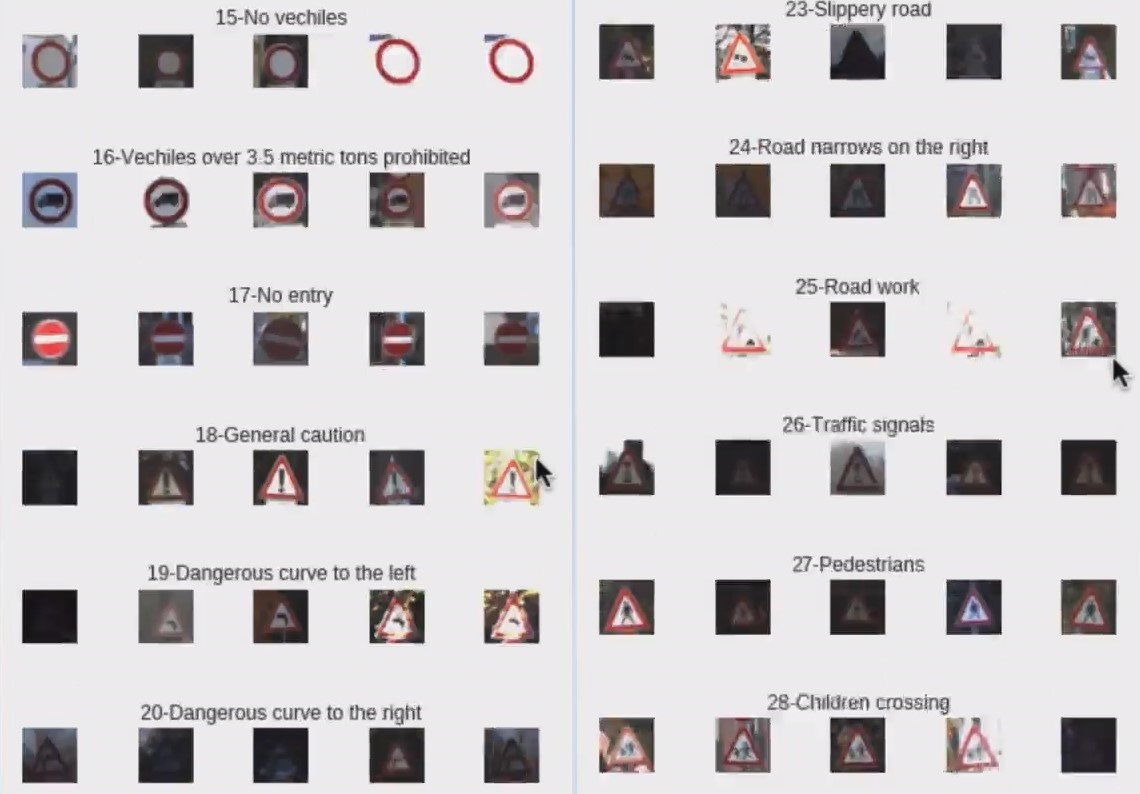
\includegraphics[width=0.9\textwidth]{trafikdata.jpg} % Resim dosyasının adını ve uzantısını belirtin
  \caption{Trafik İşaretleri Veri Örneği}
  \label{fig:resim_etiketi}
\end{figure}

\subsection{Davranışsal Klonlama ve Regresyon}Bu bölümde, sürekli bir spektrum temelinde direksiyon açılarını tahmin edebilen bir modeli eğiteceğim.Temel olarak bize Udacity tarafından açık kaynak olarak sağlanan bir otonom araç simülatörünü indireceğim.Simülatörü kullanarak modelim için kendi eğitim verilerimizi oluşturacağım ve simülatör içinde bir aracı eğitim pisti boyunca sürerken sürüş verilerini elde edeceğim.Her sürüş anında bu görüntüleri alacağım.Bu görüntüler, eğitim veri setimi temsil edecek ve her belirli görüntünün etiketi, aracın o belirli anındaki direksiyon açısı olacak.Daha sonra bu görüntüleri konvolüsyonel nöral ağıma gösterecek ve modelin, manuel sürücü olarak bizim davranışımızdan öğrenerek otonom bir şekilde nasıl sürüş yapacağını öğrenmesine izin vereceğim. Bu modelin öğrenmeyi ayarlamayı öğreneceği ana değişken, herhangi bir belirli anındaki aracın direksiyon açısını uygun bir derecede ayarlamayı etkili bir şekilde öğrenecektir.Modelimi eğittikten sonra performansını,arabayı otonom olarak çalıştıracağım tamamen farklı bir test pistinde değerlendireceğim.Arabayı doğru bir şekilde eğitebilirsek,ikinci pistimizde çok iyi bir performans sergileyecek ve kendi kendine sürüş yapacaktır.
\\[30pt]
\begin{figure}[h]
  \centering
  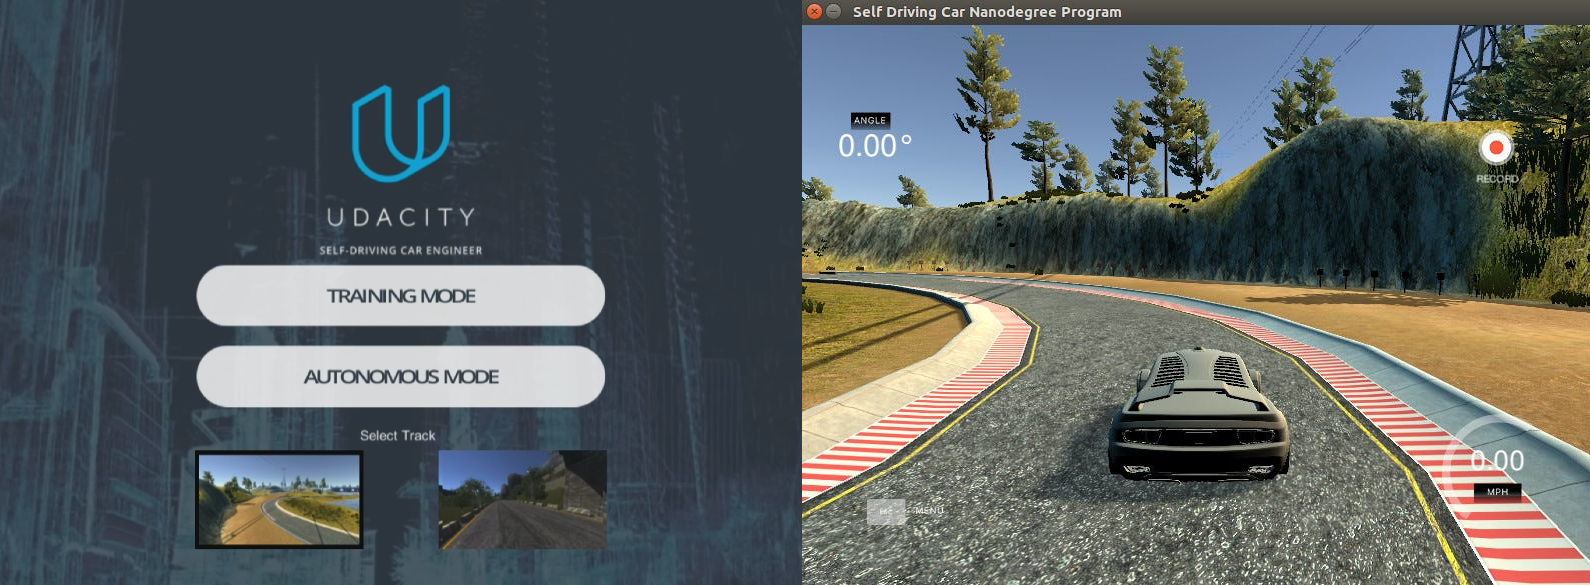
\includegraphics[width=1\textwidth]{simülatör-araba.png} % Resim dosyasının adını ve uzantısını belirtin
  \caption{Simülatör içi görüntüler}
  \label{fig:resim_etiketi}
\end{figure}

\newpage

\section{Literatür Araştırması}
\rule{\textwidth}{0.5pt}
Bu makalede\cite{ni2020survey}, derin öğrenme yöntemlerinin otonom araçlar alanında uygulanmasının teorileri ve uygulamaları üzerine son araştırmaları incelemektedir.Otonom araçlardaki temel sorunlar ve derin öğrenme yöntemlerine dayalı çözümleri, engel tespiti, sahne tanıma, şerit tespiti, navigasyon ve rota planlama gibi konular analiz edilir.\\[15pt]

\noindent Bu makalede\cite{simhambhatla2019self}, derin öğrenmenin bilgisayar görüşünü devrimlendirdiğini ve otonom araçların yeteneklerinin temel teknolojisi olduğunu belirtmektedir. Konvolüsyonel Sinir Ağları (CNN'ler), nesne tespiti görevini geliştirmek için derin öğrenme devriminin kalbinde bulunmaktadır. CNN'lere dayanan bir dizi başarılı nesne tespit sistemi önerilmiştir.\\[15pt]

\noindent Bu makalede\cite{smolyakov2018self},Udacity'den alınan verilerle eğitilen bir sinir ağı sürümü ve kendi topladıkları (simüle edilmiş) verilerle eğitilen özel sürümlerinin karşılaştırması yapılıyor.\\[15pt]

\section{Referanslar}
\rule{\textwidth}{0.5pt}
GitHub -\url{https://github.com/woges/UDACITY-self-driving-car/tree/master/term1_project3_behavioral_cloning}\\[5pt]
GitHub -\url{https://github.com/SakshayMahna/P4-BehavioralCloning}\\[5pt]
GitHub -\url{https://github.com/llSourcell/How_to_simulate_a_self_driving_car}\\[5pt]
GitHub -\url{https://github.com/naokishibuya/car-behavioral-cloning}\\[5pt]
GitHub -\url{https://github.com/udacity/self-driving-car-sim}\\[5pt]
Kaggle-\url{https://www.kaggle.com/datasets/aslanahmedov/self-driving-carbehavioural-cloning?select=IMG}\\[5pt]
\newpage

\section{Beklenen Sonuçlar}
\rule{\textwidth}{0.5pt}
Proje, derin sinir ağları ve konvolüsyonel sinir ağları kullanarak sürücülük davranışını klonlamak için başarıyla bir model geliştirmiştir.Elde edilen sonuçlar, eğitilen modelin pistte başarıyla sürüş yapabilme yeteneğini değerlendirmektedir.Modelin pistte ne kadar başarılı olduğu, doğrulama ve test aşamalarında elde edilen sonuçlarla belirlenir.Proje, modelin performansını optimize etmek için çeşitli parametre ayarlarının nasıl yapıldığını inceler.Bu ayarlamaların,modelin pistteki performansını artırıp artırmadığı değerlendirilir.Konvolüsyonel sinir ağlarının mekansal özellikleri, zaman serisi özelliklerinin ise rekürrent sinir ağlarıyla elde edildiği modelin başarısını inceler.Bu yaklaşımın, modelin performansını artırmada etkili olup olmadığı değerlendirilir.Proje, gerçek dünya verileriyle simülatör verilerinin birleştirilmesinin modelin eğitimine nasıl bir etki yaptığını araştırır.Bu yöntemin, modelin gerçek dünyadaki genelleme yeteneğini artırıp artırmadığı değerlendirilir.Bu sonuçlar, projenin modelin performansını ve gerçek dünyada uygulanabilirliğini değerlendirmesine olanak tanır.Ayrıca, derin öğrenme ve otonom araç teknolojilerinin gelecekteki gelişimine katkı sağlayacak bilgiler sunar.\\[15]

\begin{figure}[h]
  \centering
  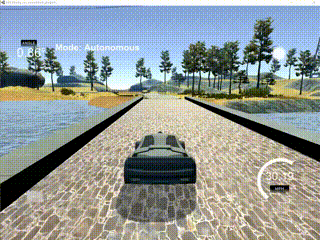
\includegraphics[width=1\textwidth]{gif.png} % Resim dosyasının adını ve uzantısını belirtin
  \caption{Otomatik modda sürüş}
  \label{fig:resim_etiketi}
\end{figure}



\bibliographystyle{ieeetr}
\bibliography{referance}



	
\end{document}
